\section{Ejercicio 4: Tiempos de propagaci\'on en compuerta CMOS}


\subsection{Descripci\'on del an\'alisis}
Se estudia en esta secci\'on, el comportamiento de una compuerta CMOS, en particular la 74HC02, una compuerta NOR, con el fin de estudiar las diferencias de las respuestas temporales de las mismas con y sin carga. Para ello se analizan los tiempos de propagaci\'on$(t_P)$, en las transiciones de alto a bajo y de bajo a alto, y el \textit{rise time}$(t_R) $y \textit{fall time}$(t_F)$ bajo estas condiciones.

Adem\'as se estudia el comportamiento de esta compuerta a altas frecuencias, 100KHz, y los efectos que puede ocasionar en la fuente de alimentaci\'on. Por \'ultimo, se agrega entre los terminales de alimentaci\'on de la compuerta, un capacitor de desacople con el fin de analizar sus efectos al trabajar en estas frecuencias.

Se muestra en la Figura \ref{fig:LOAD_CIRC} el circuito utilizado  para todo el an\'alisis.
\begin{figure}[H]
    \centering
    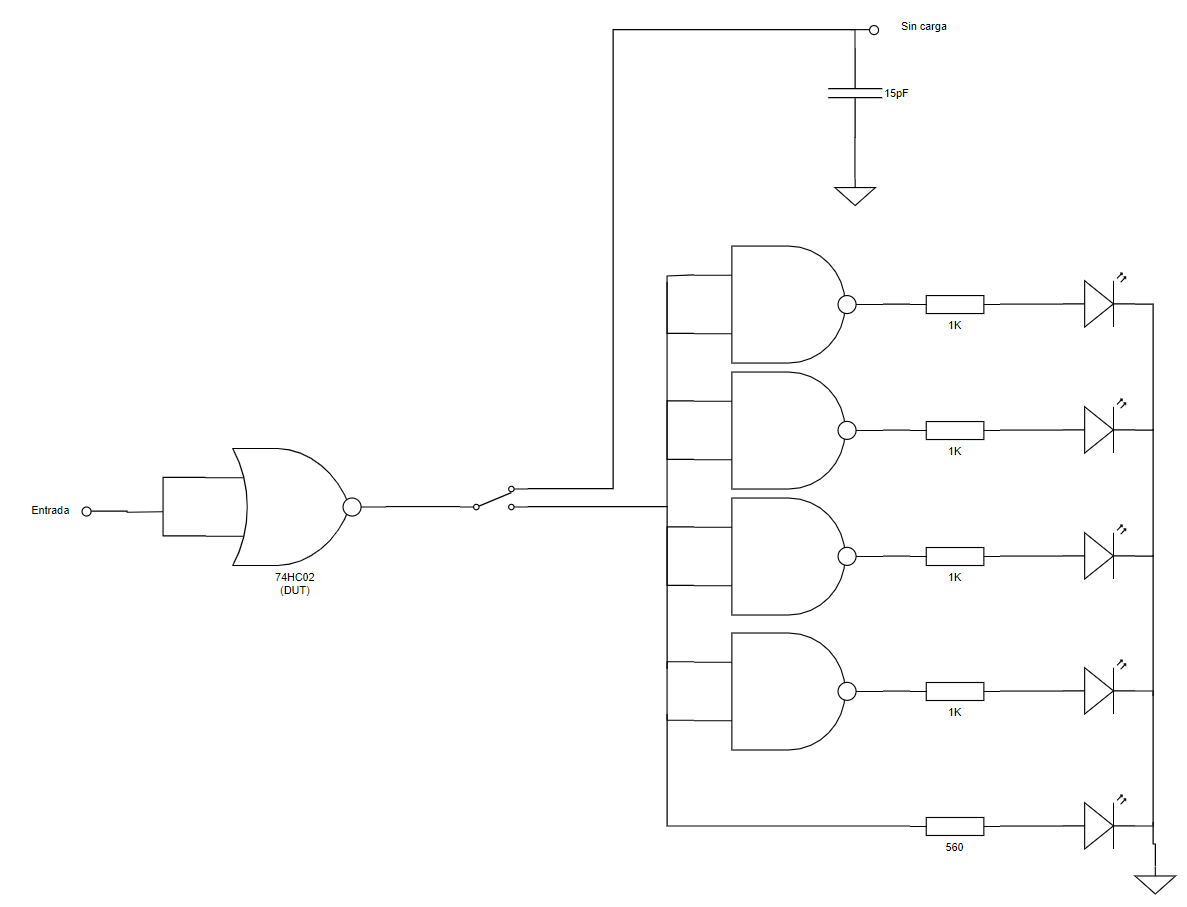
\includegraphics[width=0.8\textwidth]{../EJ4/Recursos/LOAD_CIRC}
    \caption{Circuito de medici'on}
    \label{fig:LOAD_CIRC}
\end{figure}

\subsection{Resultados}

\subsubsection{Mediciones de tiempo de propagaci\'on}
Se pueden observar en la Figura \ref{fig:PROP_NOLOAD} las mediciones obtenidas en el osciloscopio de los tiempos de propagaci\'on en ambas transiciones de la compuerta. En la Figura \ref{fig:PROP_LOAD} se muestran las mediciones equivalentes para el caso con el circuito cargado.
Se puede apreciar en las figuras, el m\'etodo de medici\'on utilizado para estos par\'ametros, por medio de cursores.
\begin{figure}[H]
    \centering
    \begin{tabular}{c c}
        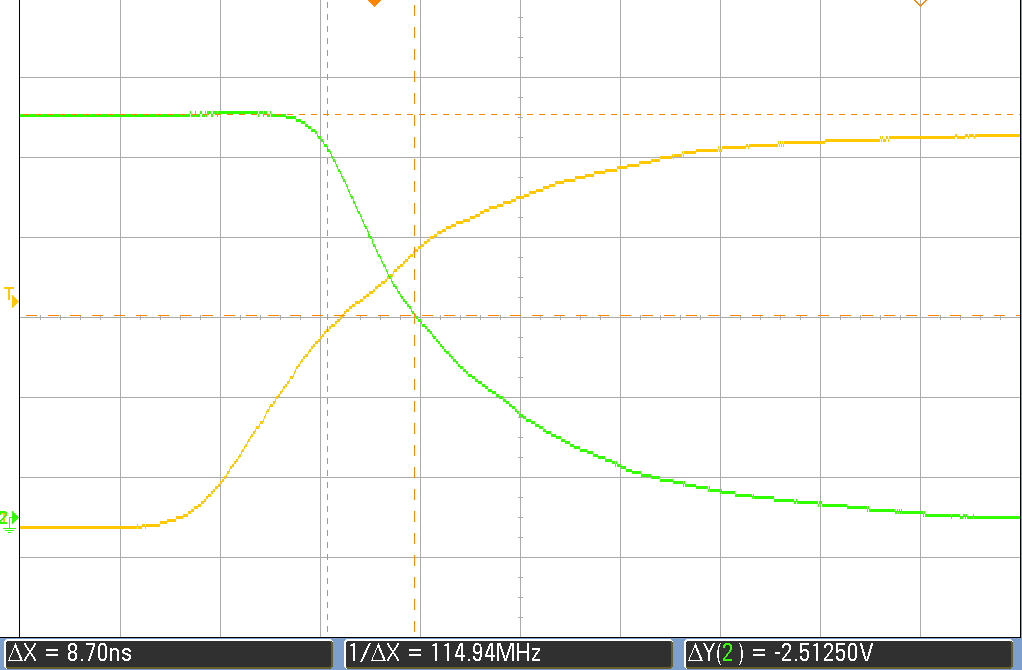
\includegraphics[width=0.4\textwidth]{../EJ4/Recursos/PROP_NOLOAD_FALL} &
        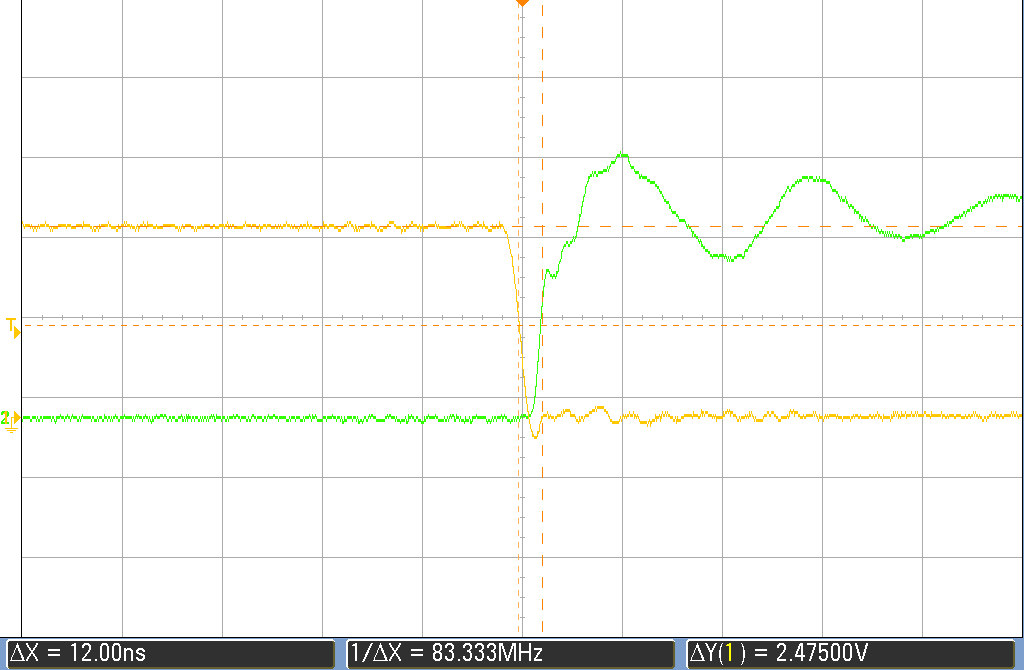
\includegraphics[width=0.4\textwidth]{../EJ4/Recursos/PROP_NOLOAD_RISE}
    \end{tabular}
    \caption{Mediciones de $t_P$ sin carga. Entrada en amarillo y salida en verde}
    \label{fig:PROP_NOLOAD}
\end{figure} 
\begin{figure}[H]
    \centering
    \begin{tabular}{c c}
        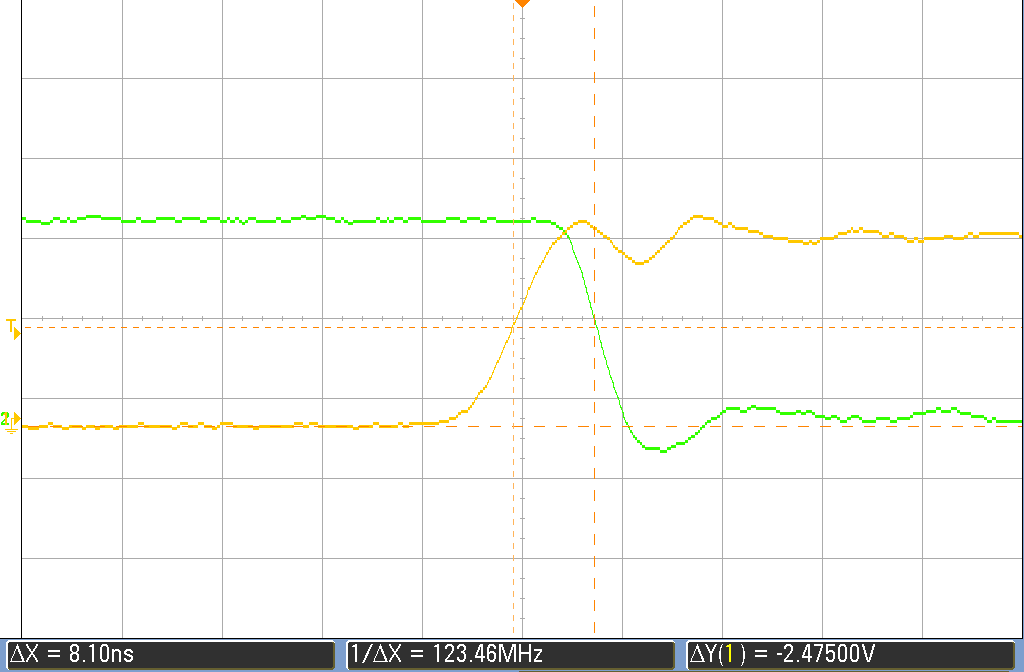
\includegraphics[width=0.4\textwidth]{../EJ4/Recursos/PROP_LOAD_FALL} &
        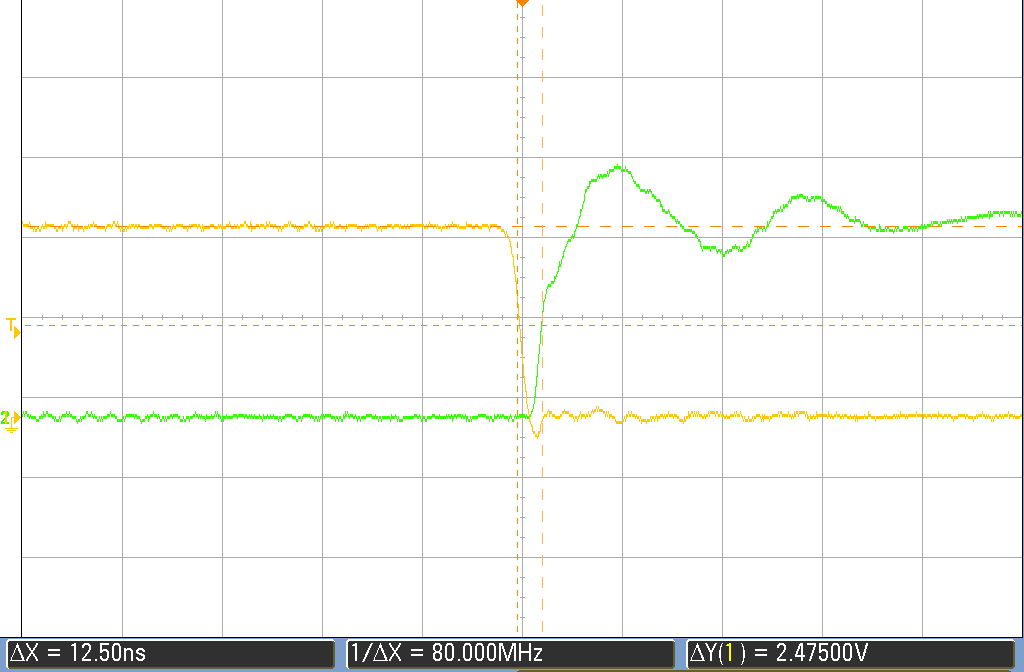
\includegraphics[width=0.4\textwidth]{../EJ4/Recursos/PROP_LOAD_RISE}
    \end{tabular}
    \caption{Mediciones de $t_P$ con carga. Entrada en amarillo y salida en verde}
    \label{fig:PROP_LOAD}
\end{figure} 
Se presenta en la Tabla \ref{tab:COMP_TP} una comparaci\'on de las mediciones realizadas.
\begin{table}[H]
    \centering
    \resizebox{0.4\textwidth}{!}{%
    \begin{tabular}{ccc}
    \hline
    $t_P$ & Fall{[}ns{]} & Rise{[}ns{]} \\ \hline
    Sin carga & 8.7 & 12 \\
    Cargado & 8.1 & 12.5 \\ \hline
    \end{tabular}%
    }
    \caption{Tabla de comparaci\'on de tiempos de propagaci\'on medidos}
    \label{tab:COMP_TP}
    \end{table}
De las mediciones, no se puede observar una diferencia significativa. Sin embargo, si se decide hacer una menci\'on acerca del sobrepico o \textit{overshoot} que se observa en las capturas tomadas. Sobre este se hace una menci\'on con mayor profundidad en las siguientes secciones.


\subsubsection{Mediciones de tiempo rise y fall}
Se pueden observar en la Figura \ref{fig:TRAN_NOLOAD} las mediciones obtenidas en el osciloscopio de los tiempos de rise y fall  de la compuerta. En la Figura \ref{fig:TRAN_LOAD} se muestran las mediciones equivalentes para el caso con el circuito cargado.
A diferencia del caso anterior,para realizar la medici\'on, se decide utilizar la funci\'on provista por el osciloscopio utilizado. Las im\'agenes que corresponden a la transici\'on de la salida de 1 a 0, se encuentran invertidas debido a que solo es posible medir con este m\'etodo, el tiempo de rise.
\begin{figure}[H]
    \centering
    \begin{tabular}{c c}
        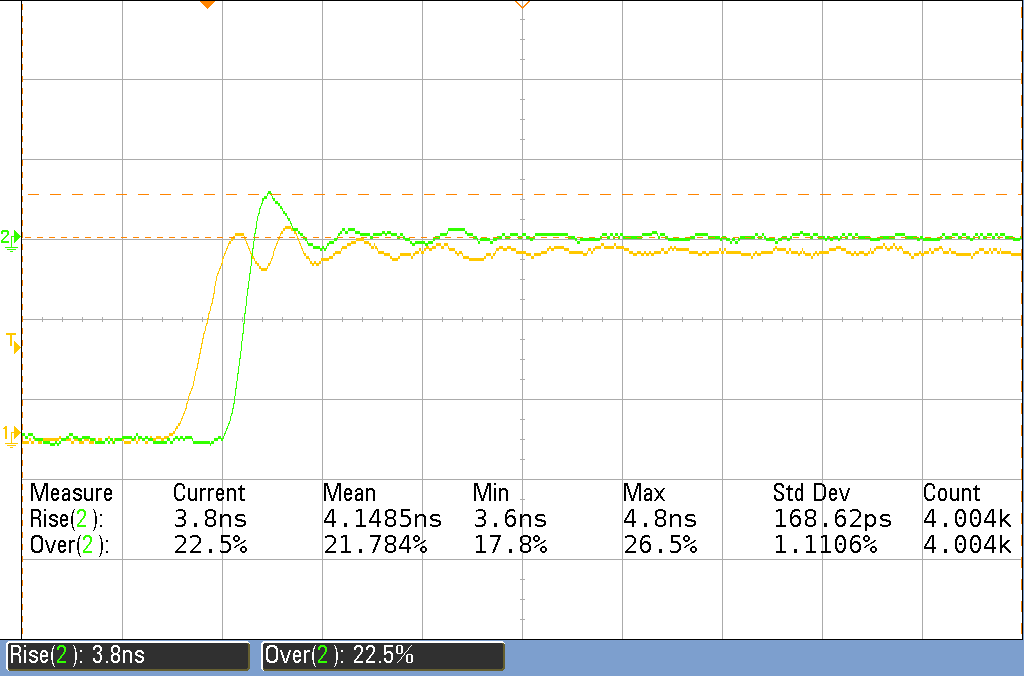
\includegraphics[width=0.4\textwidth]{../EJ4/Recursos/TRAN_NOLOAD_FALL} &
        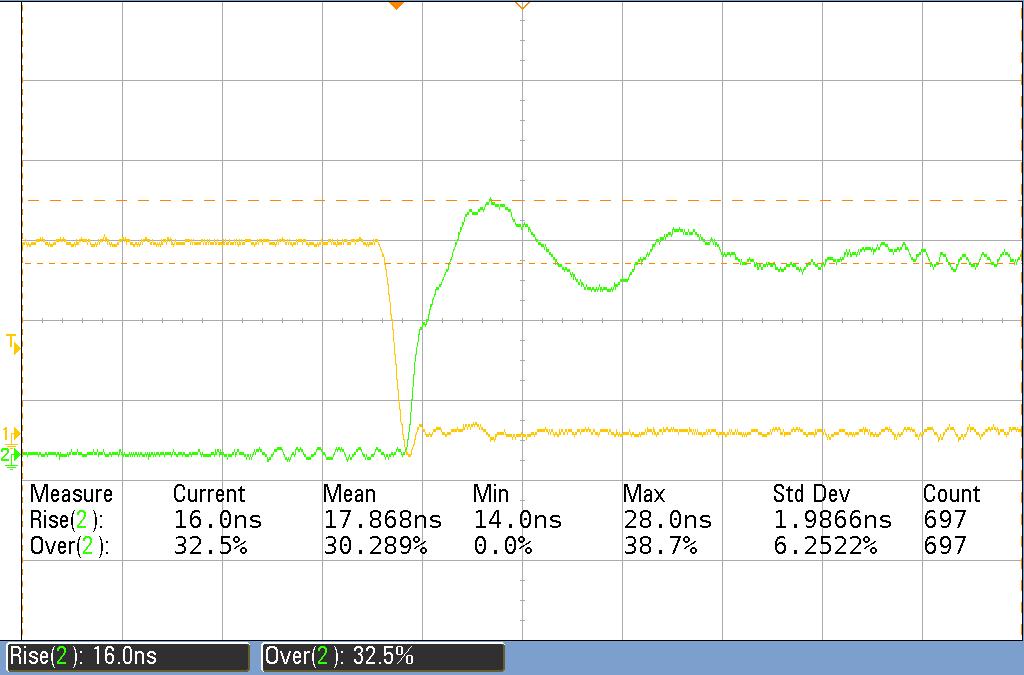
\includegraphics[width=0.4\textwidth]{../EJ4/Recursos/TRAN_NOLOAD_RISE}
    \end{tabular}
    \caption{Mediciones de $t_F$ (izquierda) y $t_R$ (derecha) sin carga. Entrada en amarillo y salida en verde}
    \label{fig:TRAN_NOLOAD}
\end{figure} 
\begin{figure}[H]
    \centering
    \begin{tabular}{c c}
        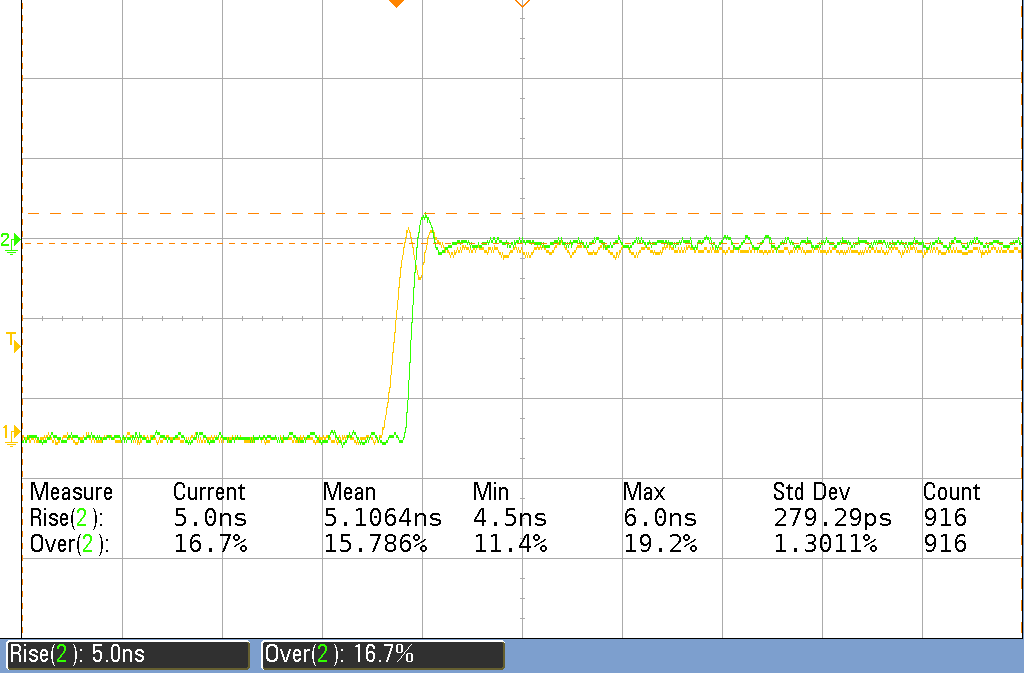
\includegraphics[width=0.4\textwidth]{../EJ4/Recursos/TRAN_LOAD_FALL} &
        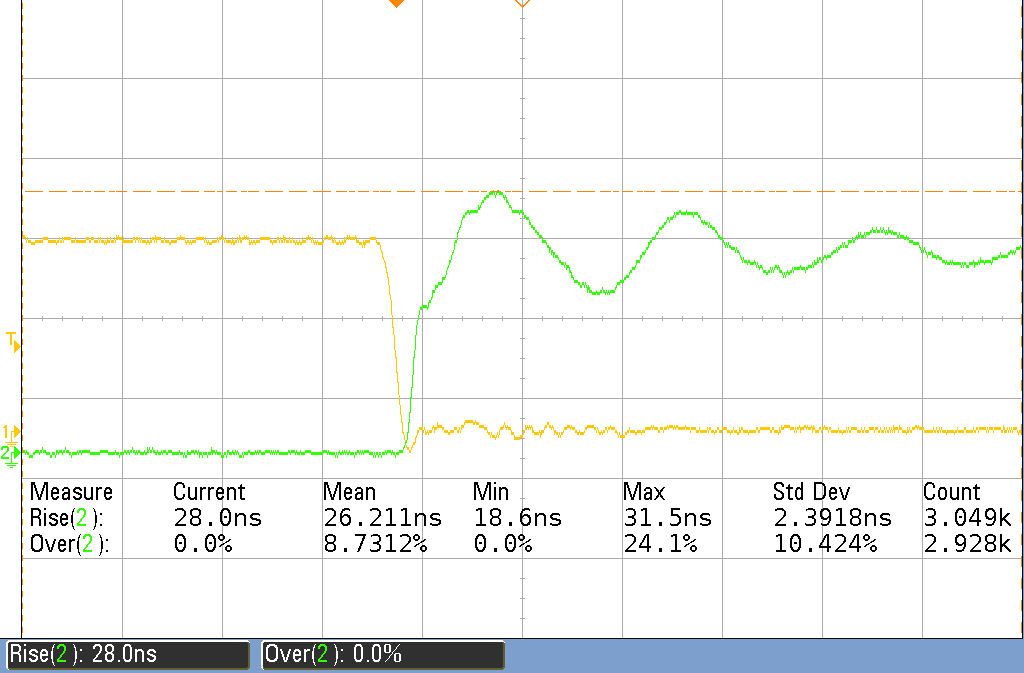
\includegraphics[width=0.4\textwidth]{../EJ4/Recursos/TRAN_LOAD_RISE}
    \end{tabular}
    \caption{Mediciones de $t_F$ (izquierda) y $t_R$ (derecha) con carga. Entrada en amarillo y salida en verde}
    \label{fig:TRAN_LOAD}
\end{figure}
Se presenta en la Tabla \ref{tab:COMP_TR_TF} una comparaci\'on de las mediciones realizadas de los tiempos mencionados.
\begin{table}[H]
    \centering
    \resizebox{0.4\textwidth}{!}{%
    \begin{tabular}{ccc}
    \hline
    $t$ & Fall{[}ns{]} & Rise{[}ns{]} \\ \hline
    Sin carga & 4.14 & 17.86 \\
    Cargado & 5.1 & 26.11 \\ \hline
    \end{tabular}%
    }
    \caption{Tabla de comparaci\'on de tiempos de fall y rise medidos}
    \label{tab:COMP_TR_TF}
    \end{table}
En esta medici\'on si se encuentra una variaci\'on significativa al comparar los tiempos con y sin carga, en especial en los tiempos de rise. Esto se debe a que, al conectar m\'as compuertas l\'ogicas a la salida, la capacidad equivalente a la salida de la compuerta NOR es mayor.

Un punto importante a remarcar es que, los tiempos de fall medidos, se encuentran muy cerca del rise time del osciloscopio, que se calcula como $t_R^{OSC} = \frac{0.35}{BW} = 3.5 ns$ por lo que los valores tomados en esta medici\'on no son del todo correctos. 
\subsubsection{Overshoot}
En todas las mediciones realizadas, se puede observar en ambos flancos de transici\'on un transitorio correspodiente a un sistema subamortiguado con su respectivo \textit{overshoot} o sobrepico. Este fen\'omeno se debe principalmente a la capacidad par\'asita que se encuentra entre el drain y source de la salida de una compuerta CMOS\footnote{Fuente: https://pdfs.semanticscholar.org/f408/39a2cefd5e5a55e25fa21453d79be764a287.pdf. Consultado: 14/10/2019}. Ad\'emas, es importante considerar las influencias de las puntas del osciloscopio en el circuito, al cambiarlas de x10 a x1 se observa que desaparece el sobrepico.


\subsubsection{Mediciones a altas frecuencias}
Para realizr este an\'alisis se aumenta la frecuencia del generador de se\~nales a 100KHz y se miden los efectos que esto produce en la alimentaci\'on.
Se muestran en la Figura \ref{fig:DC_NOCAP} los resultados obtenidos.
\begin{figure}[H]
    \centering
    \begin{tabular}{c c}
        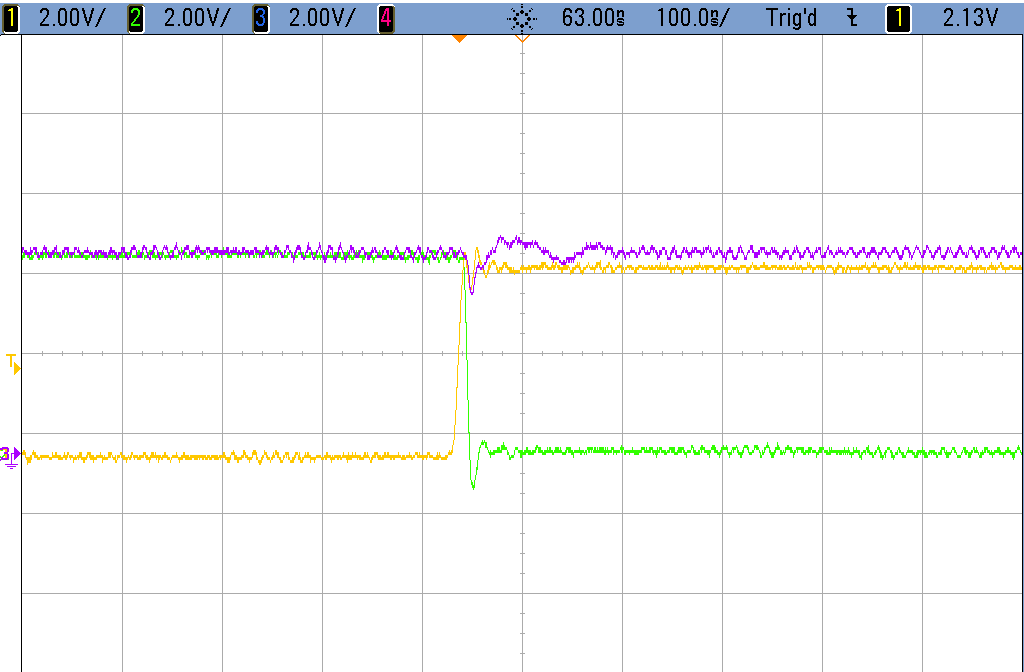
\includegraphics[width=0.4\textwidth]{../EJ4/Recursos/DC_VAR_FALL} &
        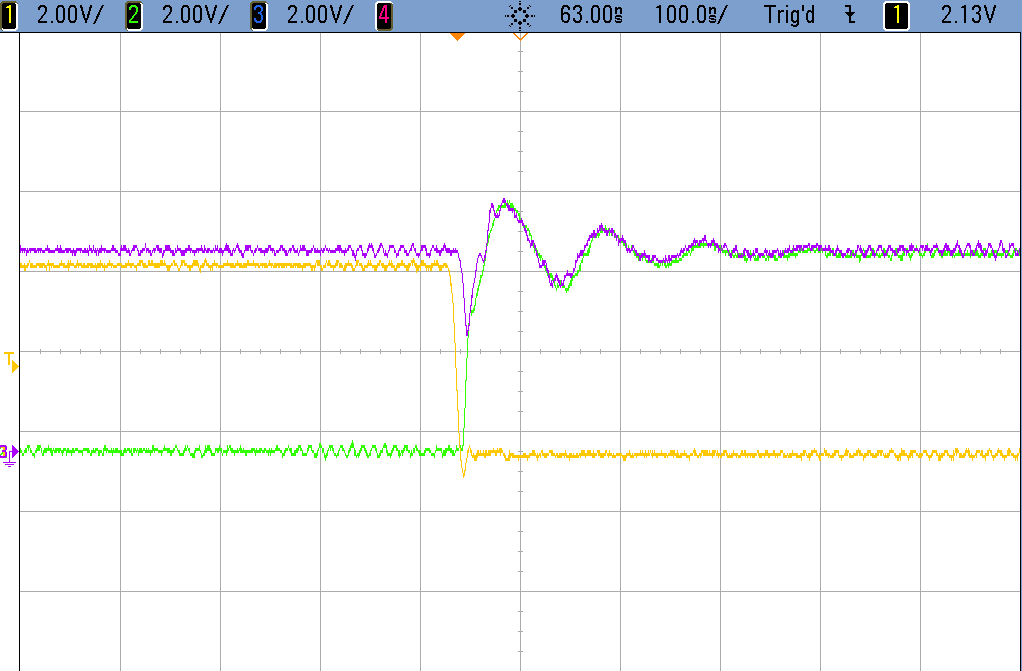
\includegraphics[width=0.4\textwidth]{../EJ4/Recursos/DC_VAR_RISE}
    \end{tabular}
    \caption{Mediciones de la alimentaci\'on a 100KHz. Entrada en amarillo, salida en verde y alimentacion en violeta}
    \label{fig:DC_NOCAP}
\end{figure}

Se observa que la alimentaci\'on tiene un transitorio subamortiguado coincidente con los flancos de transici\'on de la salida. Esto se debe a que, en la transici\'on, la compuerta demanda m\'as corriente de la fuente en un per\'iodo de tiempo corto. La amplitud y per\'iodo del transitorio dependen de la respuesta en frecuencia de la fuente utilizada. 

Debido a este sobrepico, la tensi\'on de alimentaci\'on cae por debajo de los 3V, cuando el m\'inimo se\~nalado por el fabricante es de 2V, y sube casi llegando a los 6V, el m\'aximo \footnote{Fuente:http://www.ti.com/lit/ds/symlink/sn74hc02.pdf. Consultado: 14/10/2019}. Esto es sumamente cr\'itico pues el comportamiento del circuito es incierto.

Para solucionar esto, se agrega entre los terminales de alimentaci\'on de la compuerta, un capacitor de desacople de 100nF. La selecci\'on de ese valor se realiza en base a lo especificado por Texas Instruments en la "Gu\'ia de consideraciones de dise\~no para dispositivos l\'ogicos"\footnote{Fuente:https://www.ti.com/lit/an/sdya002/sdya002.pdf. Consultado: 14/10/2019}
Se muestran en la Figura \ref{fig:DC_CAP} los resultados obtenidos.
\begin{figure}[H]
    \centering
    \begin{tabular}{c c}
        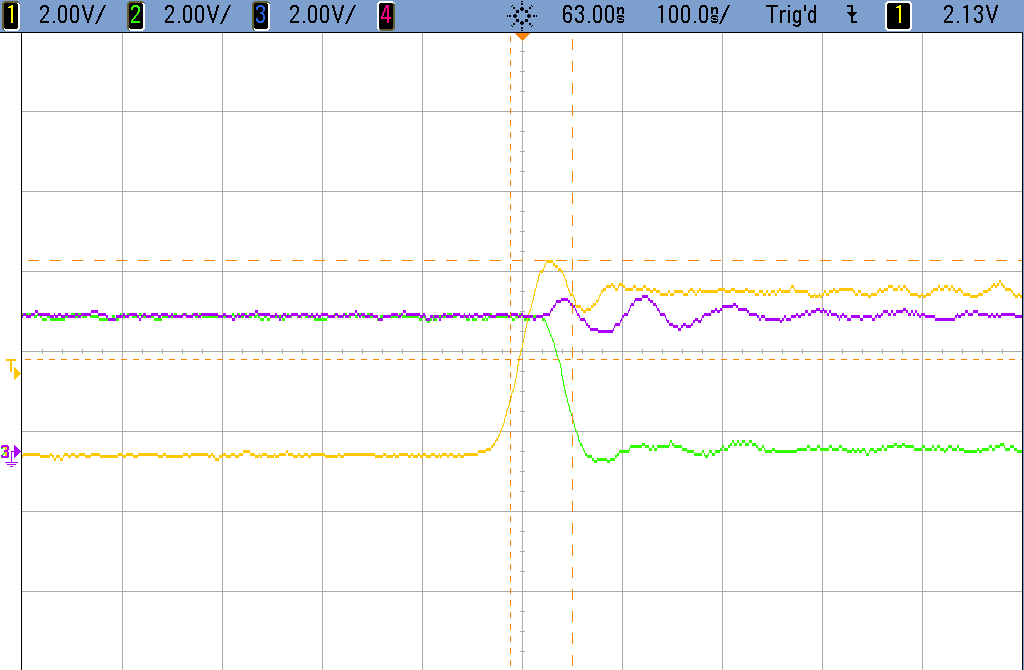
\includegraphics[width=0.4\textwidth]{../EJ4/Recursos/DC_VAR_FALL_CAP} &
        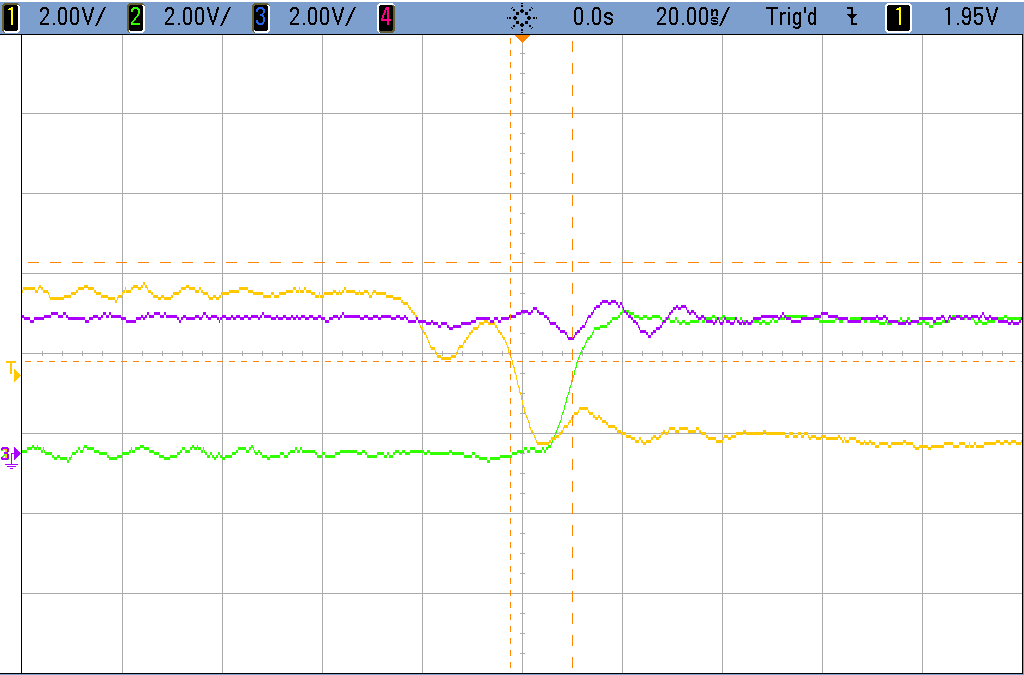
\includegraphics[width=0.4\textwidth]{../EJ4/Recursos/DC_VAR_RISE_CAP}
    \end{tabular}
    \caption{Mediciones de la alimentaci\'on a 100KHz con capacitor de desacople. Entrada en amarillo, salida en verde y alimentacion en violeta}
    \label{fig:DC_CAP}
\end{figure}

Los resultados se corresponden con lo esperado. Se puede observar en las capturas que, si bien el transitorio sigue presente, el sobrepico tiene una amplitud mucho menor.  

En cuanto a la temperatura, no se observaron variaciones al aumentar la frecuencia de operaci\'on.

\subsection{Conclusi\'on}
Se ha podido comprobar la influencia que tiene la carga conectada a una compuerta en sus tiempos caracter\'isticos. Adem\'as se pudo observar las asimetr\'ias en los tiempos de rise y fall provocadas por los transistores a la salida de la compuerta.
Por \'ultimo, se destaca a partir de los resultados la importancia de utilizar capacitores de desacople en la implementacion de circuitos l\'ogicos para asegurar su correcto funcionamiento.